% !TeX spellcheck = it_IT
Negli ultimi anni, un numero sempre crescente di infrastrutture critiche è stato digitalizzato, aggiungendo capacità di comunicazione e di computazione a numerosi dispositivi nelle reti di distribuzione dell'energia e dell'acqua, sistemi di trasporto, e manifatturieri. Ciò avviene in parte con lo scopo di aumentare l'efficienza, ma spesso è anche un requisito necessario a gestire l'ambiente che muta, come ad esempio la generazione locale dell'energia o il passaggio ai veicoli elettrici nel caso della distribuzione energetica.\\
Un progetto di digitalizzazione molto visibile è il passaggio dai \emph{meter} analogici ai digitali (\emph{smart}), che è attualmente in corso in vari paesi del mondo. Oltre ad una fatturazione complessivamente più precisa, uno smart meter può anche dare input agli algoritmi di controllo della grid, essere usato nei mercati energetici, comunicare con la \emph{smart home} (ad esempio, per regolare l'aria condizionata ed i sistemi di riscaldamento quando la richiesta energetica è alta), oppure per disconnettere da remoto un consumatore. In questo modo, un dispositivo precedentemente disconnesso e non critico si trasforma in un dispositivo connesso che può generare dati \emph{process-critical}.\\
La robustezza dei dati e dei comandi di switch è vitale - se una grande quantità di famiglie viene disconnessa simultaneamente, l'energia in eccesso non ha dove andare, potrebbe danneggiare la grid. In maniera simile, se gli algoritmi di manutenzione si basano su dati provenienti da misure effettuate dagli smart meter, input errati possono produrre effetti di gran lunga peggiori delle frodi di fatturazione. Ciò pone una nuova sfida per i produttori di meter: progettare dispositivi economici, largamente distribuiti e che lavorino su canali con banda molto ristretta.
\section{Open Smart Grid Protocol}
L'Open Smart Grid Protocol (OSGP) è stato uno dei primi protocolli di comunicazione su powerline per smart meters disponibile sul mercato, ed è largamente utilizzato per comunicare tra smart meter e l'aggregatore di dati, il quale è un dispositivo che colleziona dati provenienti da diverse centinaia di meter in un segmento di PLC (Power Line Communication) e li inoltra ad un controllore centralizzato.\\
L'OSGP risiede nel layer delle applicazioni dello stack protocollare definito dallo standard 14908 ISO/IEC \cite{standard14908}. Nonostante l'OSGP sia principalmente utilizzato per applicazioni di smart-metering, esso è stato progettato per un utilizzo più ampio all'interno di dispositivi della Smart Grid. Lo stack protocollare è molto leggero. Tale leggerezza è ottenuta pagando in sicurezza, infatti le primitive crittografiche consigliate dal NIST  (ad esempio: Advanced Encryption Standard - AES, in \emph{authenticated mode}) sono evitate, optando per altre meno intense computazionalmente: lo stream cipher RC4 per la cifratura ed una funzione digest non standard per l'autenticazione dei messaggi.\\
Il problema più grande è la combinazione di uno stream cipher con una funzione di digest lineare, che apre le possibilità per attacchi alle chiavi crittografiche ed ai messaggi. Ad esempio, si potrebbe sfruttare tale vulnerabilità utilizzando il ricevente di un messaggio come un ``oracolo". Dato un messaggio propriamente cifrato ed autenticato, un attaccante ipotizza una combinazione di un bit del messaggio ed un bit della chiave, invia un messaggio, appositamente confezionato, al ricevente ed utilizza la risposta del  dispositivo che rifiuti o confermi l'ipotesi. Siccome questo può essere effettuato per singoli bit, un attaccante può ricostruire la chiave principale del dispositivo (OMA key) con al più $96 \times 3$ risposte.
\subsection{Potenziali debolezze del protocollo}
Sono state identificate quattro potenziali debolezze nel protocollo OSG.
\subsubsection{Utilizzo di RC4}
Negli ultimi anni sono state identificate varie debolezze nello stream cipher RC4. Uno dei problemi è la correlazione tra la chiave ed il \emph{keystream} di RC4 che può essere utilizzata per ricostruire la chiave. Questa debolezza è stata sfruttata con successo attraverso i vettori di inizializzazione (IVs)  utilizzati per ``rompere" WEP (Wired Equivalent Protection), standard che fa largo uso di RC4. Gli attacchi \cite{wep1}, \cite{wep2} rompono WEP in pochi secondi e tool per l'attacco come Aircrack-ng \cite{aircrackng} sono disponibili gratuitamente per effettuare penetration testing \cite{kali}.\\
L'uso di RC4 nel protocollo OSG è simile al modo in cui RC4 era usato nello standard WEP. Mentre, per ogni messaggio, è generata una nuova chiave, solamente i primi 8 byte della chiave variano, ed i restanti 8 byte sono costanti. Inoltre, gli 8 byte iniziali vengono messi in XOR con un valore noto pubblicamente. Sebbene gli autori non siano a conoscenza di un attacco reale a tale caratteristica, ciò implica una forte correlazione tra le chiavi usate, e fornisce ad un attaccante dati interessanti da analizzare. Ulteriormente, l'impostazione è simile a quella utilizzata nello standard WEP, questo lascia intuire che l'esperienza nel campo dello \emph{statistical key recovery} permetterebbe di attuare con successo un attacco.\\
Un altro problema di RC4 in OSGP è che è utilizzato con una autenticazione debole. Data la natura di uno stream cipher, un attaccante che entra in possesso di un \emph{ciphertext} può alterare bit in posizioni scelte. Grazie alla conoscenza dello spazio dei messaggi dello standard EN 14908, un attaccante può inviare messaggi alterati che sono validi con alta probabilità. Inoltre, egli può autenticare tali messaggi sfruttando la debolezza della funzione di digest descritta qui di seguito.
\subsubsection{Debole funzione di digest}
La funzione di digest utilizzata nel protocollo OSG per l'autenticazione dei messaggi è lineare ed è implementata in un modo che non solo disabilita l'autenticazione ma può inoltre lasciar decifrare un messaggio intercettato in tempo lineare nella lunghezza del messaggio. La debolezza strutturale intrinseca alla funzione di digest consente un attacco ``man-in-the-middle" (che dimezza la taglia della chiave per un attacco di forza bruta), la modifica dei messaggi in maniera controllata, ricomputazione del digest corretto senza il bisogno di cifratura - o di chiavi di autenticazione, ed utilizzando i messaggi di NACK di un dispositivo su un digest errato per ricostruire sia la chiave di autenticazione che il messaggio.
\subsubsection{Sicurezza di broadcast non definita}
Nonostante la funzione di broadcast sia chiamata ``Secure Broadcast", la sicurezza definita su di essa è molto bassa. Questo è particolarmente preoccupante, se si pensa che tale meccanismo è utilizzato per inviare aggiornamenti del firmware, che sono distribuiti attraverso il meccanismo di broadcast sicuro senza alcuna misura specifica atta a fornire autenticazione dalla sorgente.
\subsubsection{Utilizzo della chiave}
Sebbene il protocollo faccia uso di chiavi di sessione per la cifratura, utilizza una master key per l'autenticazione. Comunque, questa chiave di autenticazione è usata per derivare la cifratura delle chiavi di sessione. Quindi se la chiave di autenticazione è compromessa, tutte le chiavi di sessione sono note dall'attaccante. Siccome la chiave di autenticazione è usata con un debole algoritmo di autenticazione, essa è altamente esposta ad un gran numero di attacchi, e comprometterla è ben possibile.
\subsection{Sfruttare le debolezze strutturali}
Queste debolezze strutturali possono essere sfruttate in vari modi. Gli attacchi adatti a tale scopo complessivamente non sono molto sofisticati, piuttosto, grazie alla debolezza dei \emph{building block} crittografici un attaccante è capace di dirottare un intero segmento PLC.\\
Un attacco relativamente semplice punta a \textit{rompere} la funzione di digest così che un attaccante possa non solo forgiare messaggi, ma - avendo ottenuto accesso ad un messaggio autentico di sufficiente lunghezza - anche ricostruire chiavi crittografiche con basso sforzo, per poi inviare falsi comandi correttamente autenticati.
%-----------------------------------------------------------------------------
%\section{Attacchi}
\section{Attacking Smart Meters and Smart Devices}
Uno dei maggiori argomenti utilizzati per mettere in sicurezza gli smart meter è che i consumatori avranno accesso fisico, e potenzialmente anche logico, a tali dispositivi. Sebbene i consumatori avessero accesso ai vecchi meter, questi ultimi non operavano utilizzando tecnologie familiari ai consumatori o a cui potessero avere accesso. A causa della prevalenza di queste tecnologie ben note, gli smart meter possono essere trattati come obiettivi tradizionali, quando ci si trova ad applicare metodologie di \emph{security testing} su di essi.\\
Di seguito vengono analizzate due tra le più comuni metodologie di security testing e come queste possano essere applicate al testing degli smart meter.

\subsection{Open Source Security Testing Methodology Manual}
Nel Gennaio 2001, in USA e Spagna, fu fondato l'Institute for Security and Open Methodologies (ISECOM): organizzazione no-profit il cui scopo è quello di fornire soluzioni pratiche per security awareness, ricerca, certificazione e business integrity. Il loro \emph{Open Source Security Testing Methodology Manual} (OSSTMM) fornisce agli utenti le metodologie per effettuare security testing. L'OSSTMM contiene sei sezioni che recensiscono un numero enorme di aspetti di sicurezza, incluse reti, dispositivi wireless, e sicurezza fisica. Per tali aspetti, è possibile applicare l'OSSTMM al security testing degli smart meter.\\
Sezioni dell'ISECOM \emph{Open Source Security Testing Methodology Manual}:
\begin{enumerate}
	\item Information Security
	\item Process Security
	\item Internet Technology Security
	\item Communications Security
	\item Wireless Security
	\item Physical Security
\end{enumerate}
Eseguire security testing in accordo all'OSSTMM richiede che ogni modulo contenuto in ogni sezione sia testato secondo sei approcci comuni al testing: dal Double Blind, in cui sia target che attaccante non abbiano informazioni prima di condurre il testing, al Tandem, dove il target e l'attaccante condividono informazioni riguardo il testing apertamente. L'approccio mostrato di seguito è quello Double Blind in quanto è quello che più si avvicina ad una situazione reale.
\subsubsection{Information Security}
In questa sezione risiedono otto moduli:
\begin{enumerate}
	\item Posture assessment
	\item Information integrity review
	\item Intelligence survey
	\item Internet document grinding
	\item Human resources review
	\item Competitive intelligence review
	\item Privacy controls review
	Information controls review
\end{enumerate}
La sezione di Information Security dell'OSSTMM si concentra su \emph{information gathering} e \emph{validation}. Dalla prospettiva di un attaccante, include l'ottenimento e la revisione di informazioni riguardo la marca e modello dello smart meter target per studiarne il funzionamento, gli standard utilizzati e determinare quali attacchi possano essere più adatti rispetto ad altri.


\subsubsection{Process Security Testing}
La seconda sezione dell'ISECOM \emph{Open Source Security Testing Methodology Manual} si concentra sull'analisi di sicurezza dei processi del target e contiene i seguenti cinque moduli:
\begin{enumerate}
	\item Posture review
	\item Request testing
	\item Reverse Request testing
	\item Guided Suggestion testing
	\item Trusted Persons testing
\end{enumerate}

La seconda sezione, quindi, si occupa di ciò che solitamente è chiamata ``social engineering". Ogni modulo punta ad ottenere informazioni da persone attraverso la coercizione e l'inganno. In relazione all'attacco di smart meter, ciò include impersonare il tecnico di una compagnia o un consumatore.\\
Con questi metodi, sarebbe possibile ottenere informazioni di valore come specifiche tecniche o amministrative, o credenziali degli utenti.

\subsubsection{Internet Technology Security Testing}
La maggior parte dei moduli applicabili al testing della sicurezza degli smart meter è contenuta nei quattordici moduli di questa sezione:
\begin{enumerate}
	\item Network Surveying
	\item Port Scanning
	\item Services Identification
	\item System Identification
	\item Vulnerability Research and Verification
	\item Internet Application Testing
	\item Router Testing
	\item Trusted Systems Testing
	\item Firewall Testing
	\item Intrusion Detection System Testing
	\item Containment Measures Testing
	\item Password Cracking
	\item Denial of Service Testing
	\item Security Policy Review
\end{enumerate}

\paragraph{Network Surveying}\mbox{}\\
Punta all'identificazione dei sistemi target accessibili in rete. Nel caso di smart meters, questi sono accessibili agli attaccanti attraverso sia reti wireless che le home area networks. In entrambi i casi, il Network Surveying consiste nell'ottenere informazioni sui target (\emph{information gathering}). 
Ciò può essere realizzato in uno dei seguenti modi: passivamente, ascoltando il traffico di passaggio sulla rete, o attivamente, facendo \emph{IP probing} in attesa di una response.\\

\begin{figure}[hbtp]
	\centering
	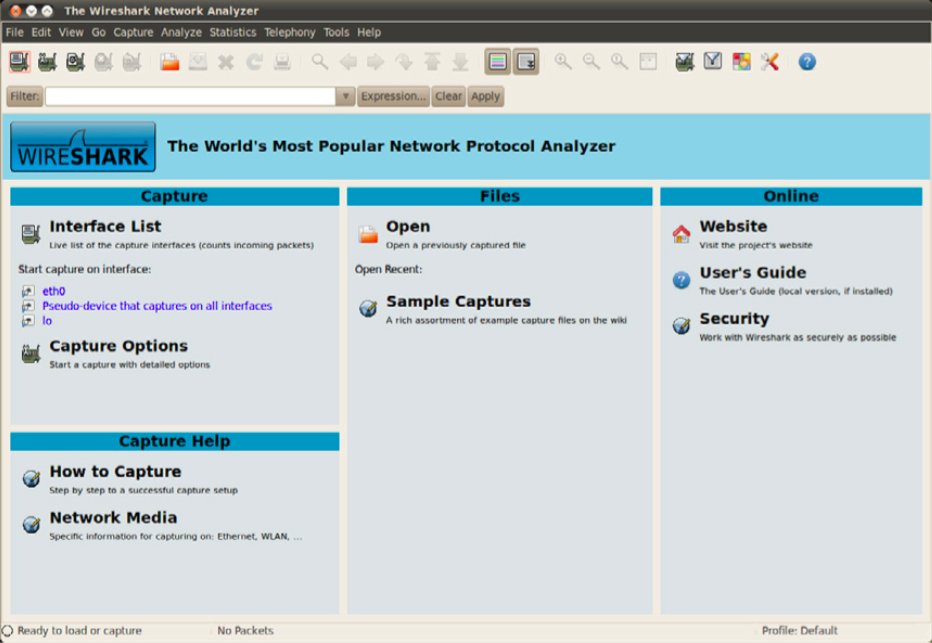
\includegraphics[scale=.3]{imgs/attack/wireshark.png}
	\caption{Wireshark sniffing tool}
	\label{wireshark_img}
\end{figure}

Per l'identificazione passiva, può essere utilizzato Wireshark, Figura \ref{wireshark_img}.\cite{wireshark} Wireshark cattura il traffico che attraversa qualsiasi rete in tempo reale e fornisce l'ispezione di centinaia di protocolli. È possibile inoltre specificare gli indirizzi IP di cui effettuare lo sniffing, così da limitare la raccolta di informazione ai possibili target.\\
Per quanto riguarda l'identificazione attiva, invece, è possibile utilizzare la tecnica del \emph{ping sweep}: essa si avvale del Internet Control Message Protocol (ICMP) per individuare i target attivi in rete analizzando le loro response. Nel caso in cui il traffico ICMP sia bloccato, è spesso utilizzato il ping di TCP. Per entrambi i casi è utilizzato il tool di sicurezza Nmap.\cite{nmap}

\paragraph{Port Scanning}\mbox{}\\
Consiste nel fare \emph{probing} sul target in attesa di risposte sulle 65,536 porte TCP e/o UDP. Ottenere una response significa che dei servizi sono in esecuzione sulle porte associate e che potrebbero contenere debolezze che esporrebbero il target. Il tool di port-scanning più utilizzato è Nmap, che permette di effettuare scan TCP completando l'\emph{handshake}, o attraverso scan TCP SYN che utilizza solamente i messaggi iniziali di SYN e SYN ACK dell'\emph{handshake} TCP.\\
L'OSSTMM suggerisce che la scelta di quali delle 65,536 porte da analizzare è a discrezione dell'attaccante e dipende dal contesto.

\paragraph{Services Identification and System Identification}\mbox{}\\
Lo scopo di questi due moduli è di enumerare i servizi in esecuzione sulle porte TCP o UDP che hanno prodotto una response nella fase di port scanning, così come identificare il sistema operativo del target.\\
Entrambi i compiti sono svolti dal tool Nmap, attivando lo switch \textbf{-sV} che fornisce informazioni addizionali ad esempio il numero di versione, come è possibile verificare nella Figura \ref{nmap_sv_img}.\\
In questo caso il target utilizzato, \emph{webserver.domain.com}, fornisce informazioni quali il sistema operativo in quanto esposte dal server web Apache. Un attaccante userebbe le informazioni ottenute per verificare la presenza di falle nelle specifiche versioni dei servizi, per poi preparare un attacco.
\begin{figure}[hbtp]
	\centering
	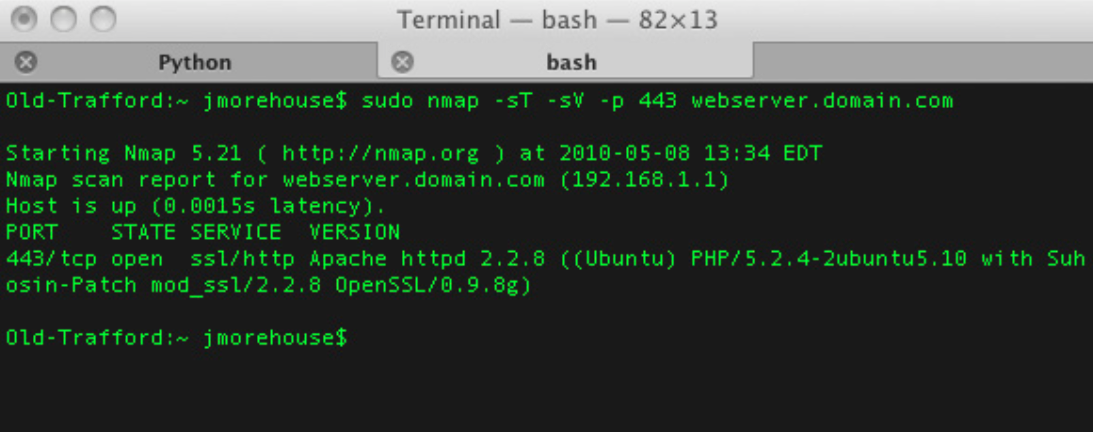
\includegraphics[scale=.3]{imgs/attack/nmap_sv.png}
	\caption{Nmap version detection ouput}
	\label{nmap_sv_img}
\end{figure}

\paragraph{Vulnerability Research and Verification}\mbox{}\\
Una volta noti sistema operativo e servizi in esecuzione con relative versioni si passa alla ricerca  e verifica di vulnerabilità tramite testing manuale ed automatizzato.\\
Un tool comunemente utilizzato per effettuare tale scan è Nessus \cite{nessus}, sviluppato dalla Tenable Network Security, mostrato in Figura \ref{nessus_img}. Sebbene Nessus sia ottimo per eseguire scanning automatizzato per determinare debolezze come una versione non aggiornata di Apache, il testing manuale dovrebbe coadiuvare quello automatizzato per individuare debolezze che potenzialmente potrebbero essere trascurate.\\
\begin{figure}[hbtp]
	\centering
	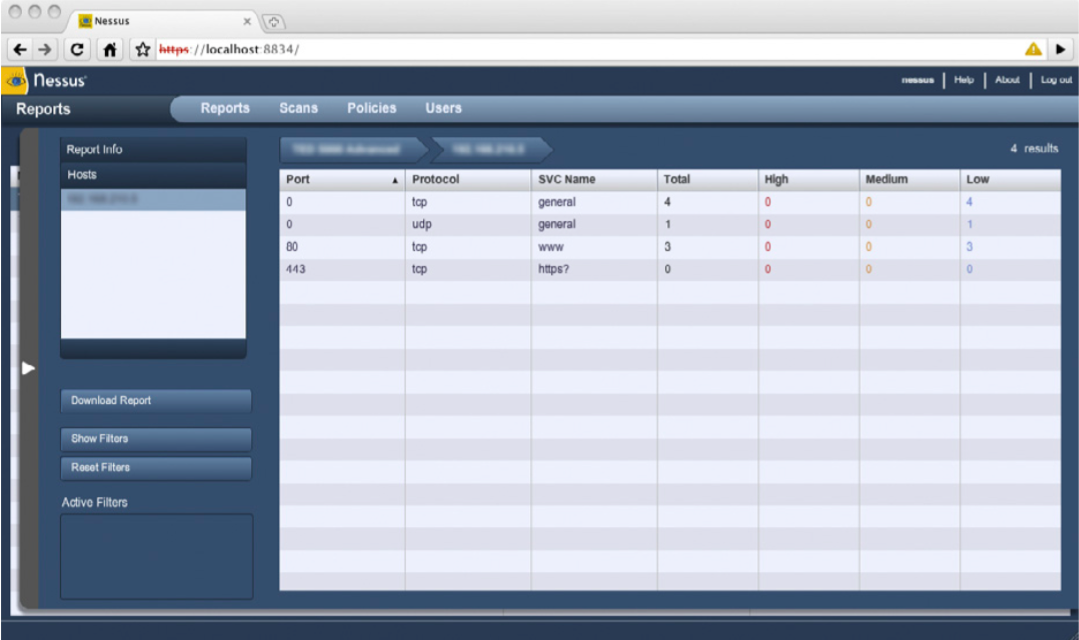
\includegraphics[scale=.3]{imgs/attack/nessus.png}
	\caption{Interfaccia web di Nessus}
	\label{nessus_img}
\end{figure}
L'OSSTMM consiglia che il testing automatizzato venga effettuato da almeno due scanner, seguito poi da una verifica manuale. Le tecniche utilizzate per la verifica manuale di vulnerabilità variano molto in funzione della vulnerabilità che si sta cercando, come ad esempio l'uso di Telnet per osservare la versione di uno specifico servizio connettendocisi, o l'utilizzo di un client FTP per connettersi ad un server FTP anonimo.\\
Nel processo di attacco a smart meter, la fase in esame è un passo critico in quanto fornisce i potenziali punti d'ingresso nello smart meter che potrebbero essere sfruttati nel modulo che segue.

\paragraph{Internet Application Testing}\mbox{}\\
Spesso, gli scanner di vulnerabilità non includono la possibilità di eseguire identificazione di vulnerabilità e verifica per Web application.\\
Con l'aumentare delle misure di sicurezza adottate dai produttori di sistemi all'interno del proprio ciclo di sviluppo, il numero di servizi in esecuzione a disposizione di attaccanti si è man mano ridotto. Ciò ha portato questi ultimi a concentrarsi sulle web application in esecuzione sui dispositivi target. Nel caso degli smart meter, tali applicazioni consentono al consumatore di visualizzare o configurare le informazioni di utilizzo, o permettono ai tecnici di configurare il dispositivo. Lo scopo di questo modulo è lo stesso del precedente, ma in un ambiente differente.\\
Effettuare identificazione e verifica di vulnerabilità su web application è significativamente più complesso che eseguire lo stesso test su servizi in esecuzione. Questo è il risultato del livello di personalizzazione trovato in ogni web application: è raro il caso che una web application sia esattamente come un'altra, ed anche nel caso di due \emph{webapp} identiche trovate in esecuzione, la loro infrastruttura di backend potrebbe differire. Per questo il testing manuale gioca un ruolo significativo e i tool a supporto di tale operazione sono molteplici. L' Open Web Application Security Project (OWASP) ha sviluppato una guida al testing per le web application, disponibile a questo indirizzo \url{https://www.owasp.org/index.php/Category:OWASP_Testing_Project}.

\paragraph{Password Cracking}\mbox{}\\
Questo modulo consiste nell'individuazione delle credenziali valide di un servizio in esecuzione o di una web application. Il testing può essere effettuato sia a partire da una lista precompilata di password, noto come attacco basato su dizionario, che provando ogni possibile combinazione di un certo alfabeto di caratteri, noto come attacco brute force.\\
Quando si esegue password cracking, è bene tenere a mente che molti servizi e web application implementano un servizio di blocco temporaneo o permanente, che disabilita un account se si verificano troppi tentativi di accesso con password invalide durante un determinato periodo di tempo.\\
Un tool comunemente utilizzato nell'ambito del password cracking, che supporti sia attacchi con dizionario che brute force, è Cain \& Abel \cite{cainabel}, mostrato in Figura \ref{cainabel_img}.\\
\begin{figure}[hbtp]
	\centering
	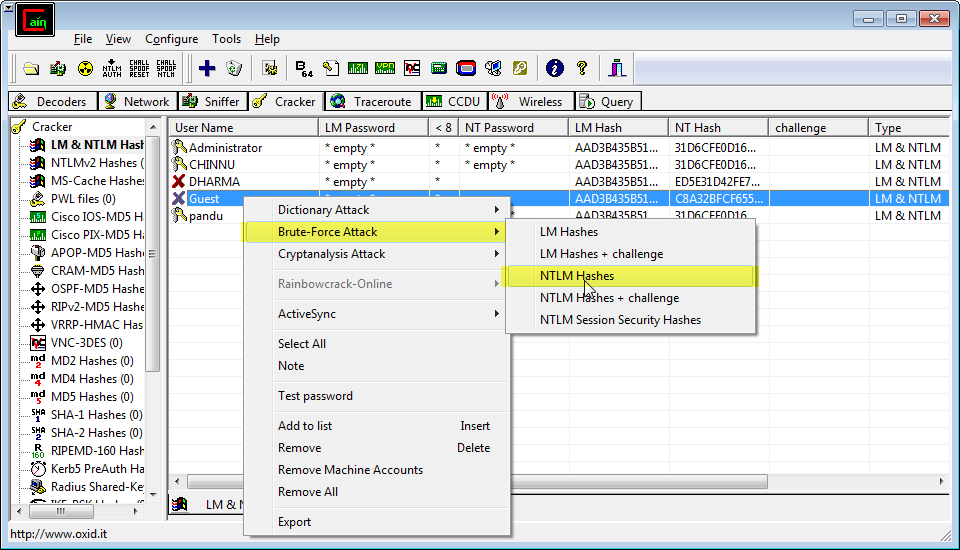
\includegraphics[scale=.3]{imgs/attack/cainabel.png}
	\caption{Il tool di password cracking Cain \& Abel}
	\label{cainabel_img}
\end{figure}
Il password cracking ha un ruolo fondamentale nell'attacco ad uno smart meter quando ci si trova davanti ad un prompt di autenticazione. Se un attaccante riesce ad ottenere le credenziali di uno smart meter, egli può istantaneamente avere accesso al dispositivo.

\paragraph{Denial of Service Testing}\mbox{}\\
Il modulo di Denial of Service si occupa di identificare i punti deboli che potrebbero essere del device stesso o all'interno dell'infrastruttura sottostante. Tale operazione potrebbe coinvolgere l'utilizzo degli strumenti precedentemente descritti, Wireshark e Nmap. Ad esempio, Wireshark potrebbe essere utilizzato per determinare i regolari pattern di traffico da e verso lo smart meter. Nmap invece potrebbe essere utilizzato per incrementare gradualmente il traffico verso lo smart meter nell'intento di sovraccaricare il dispositivo o la sua infrastruttura.\\
Se l'obiettivo dell'attaccante è semplicemente di negare il servizio ad uno smart meter, sarebbe molto semplice condurre un attacco del genere se comparato con attacchi che mirano alla compromissione della confidenzialità e/o integrità dello smart meter.

\paragraph{Exploit Testing}\mbox{}\\
Tutti i moduli descritti fin'ora gettano le basi per l'esecuzione dell'exploit testing. L'exploit testing punta ad utilizzare le vulnerabilità identificate per compromettere lo smart meter. Esempio di exploit testing includono l'utilizzo di codice per sfruttare un buffer overflow in un servizio in esecuzione o utilizzando SQL injection per accedere ad una shell di comando attraverso una falla nella validazione di un input all'interno di una web application.\\
Metasploit è un exploit tool disponibile gratuitamente che offre ai tester di sicurezza e agli attaccanti un considerevole numero di \emph{vulnerability exploit} e \emph{payload} \cite{metasploit}.
\begin{figure}[hbtp]
	\centering
	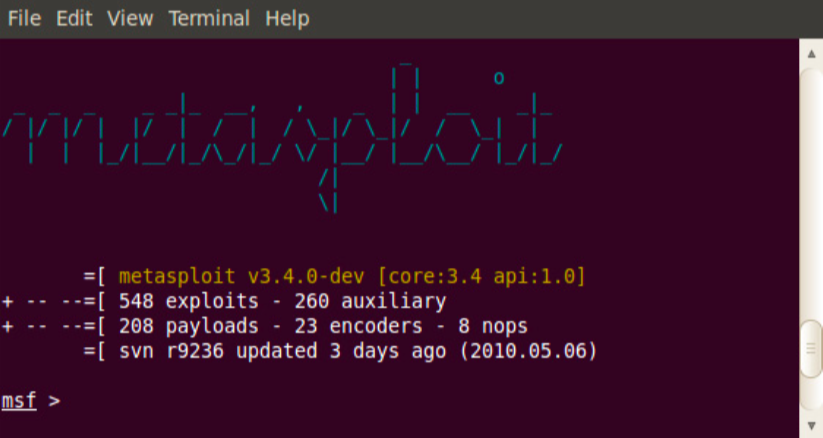
\includegraphics[scale=.3]{imgs/attack/metasploit.png}
	\caption{Il tool di vulnerability exploit Metasploit}
	\label{metasploit_img}
\end{figure}
Per un security tester, lo scopo finale è spesso quello di compromettere il target, laddove per un attaccante, la sola compromissione dello smart meter possa essere un altro passo nella propria metodologia personale di raggiungere l'obiettivo preposto.

%%%%%%%%%%%%%%%%%%%%%%%%%%%%%%%%%%%%%%%%%%%%%%%%%%%%%%%%%%%%%%%%%%%%%%%%%%%%%%%%%

\section{False Data Injection}
Nelle moderne reti di Smart Grid, la rete elettrica tradizionale è potenziata dai più recenti progressi nei campi del sensing, della misurazione e dei dispositivi di controllo con una comunicazione bidirezionale tra produttore e consumatore. La produzione di elettricità, la sua trasmissione, la distribuzione ed il consumo, scambiano informazioni sullo stato della griglia che vengono recapitate agli utenti del sistema, agli operatori ed ai dispositivi.\\
La stima dello stato ha una funzione chiave nella costruzione di modelli \emph{real-time} della rete elettrica nei centri di gestione dell'energia (EMC) \cite{monticelli}. Un modello \emph{real-time} è una rappresentazione matematica quasi statica delle attuali condizioni all'interno di una rete elettrica interconnessa. Questa rappresentazione matematica è solitamente ottenuta dai dati provenienti dalle misurazioni e dalla telemetria che avvengono a distanza di pochi secondi nel centro di controllo dell'energia (ECC). Modelli \emph{real-time} della rete possono essere utilizzati per fare scelte ottimali, rispettando vincoli tecnici come congestione delle linee di trasmissione, voltaggio e stabilità transiente. In pratica, sia economicamente che in termini di fattibilità, non è possibile misurare tutti i possibili stati nella rete; quindi, la stima dello stato è uno strumento utile per stimare tali quantità, a partire da un insieme limitato di misurazioni. Solitamente sono usati due tipi di informazione per la stima dello stato:
\begin{itemize}
	\item Dati analogici di sistemi come flussi Megavar sulle linee principali, il carico \emph{P} e \emph{Q} sui generatori e trasformatori, e i voltaggi dei bus di sistema
	\item Lo stato on/off dei dispositivi di switch come interruttori di circuito, switch di disconnessione, e tap dei trasformatori che determinano la topologia di rete
\end{itemize}
A causa dell'importanza della stima dello stato, gli effetti negativi dell'\emph{iniettare} misurazioni scorrette sono studiati in letteratura \cite{baddatainj}.  Le misurazioni scorrette possono avvenire a causa di anormalità di misura impreviste, o iniezioni dovute ad attacchi malevoli. Ad esempio, \cite{falsedatainj} è il lavoro pionieristico nello studio degli attacchi di \emph{bad data injection} che non possono essere rilevati (chiamati \emph{stealth attacks}), e mostra come un attaccante possa portare a compimento tali attacchi ``\emph{stealth}" falsificando le misure del flusso elettrico alle unità terminali remote (RTUs), manomettendo l'eterogenea rete di comunicazione o infiltrandosi all'interno del sistema della supervisione di controllo e dell'acquisizione dati (SCADA) attraverso la LAN dell'ufficio del centro di controllo. Si consideri che un sistema SCADA o un sistema di misurazione su larga area (WAMS) ottiene informazioni sulla rete elettrica (valori delle misure, stato degli interruttori, ecc.) a specifici tempi e luoghi. I centri di controllo usano le informazioni collezionate per scopi diversi, ad esempio la risoluzione di un problema di stima dello stato. In \cite{baddatainj2}, viene mostrata la fattibilità degli  attacchi di bad data injection non rilevabili, con l'obiettivo di manipolare i prezzi del mercato elettrico.
\begin{figure}[h]
	\centering
	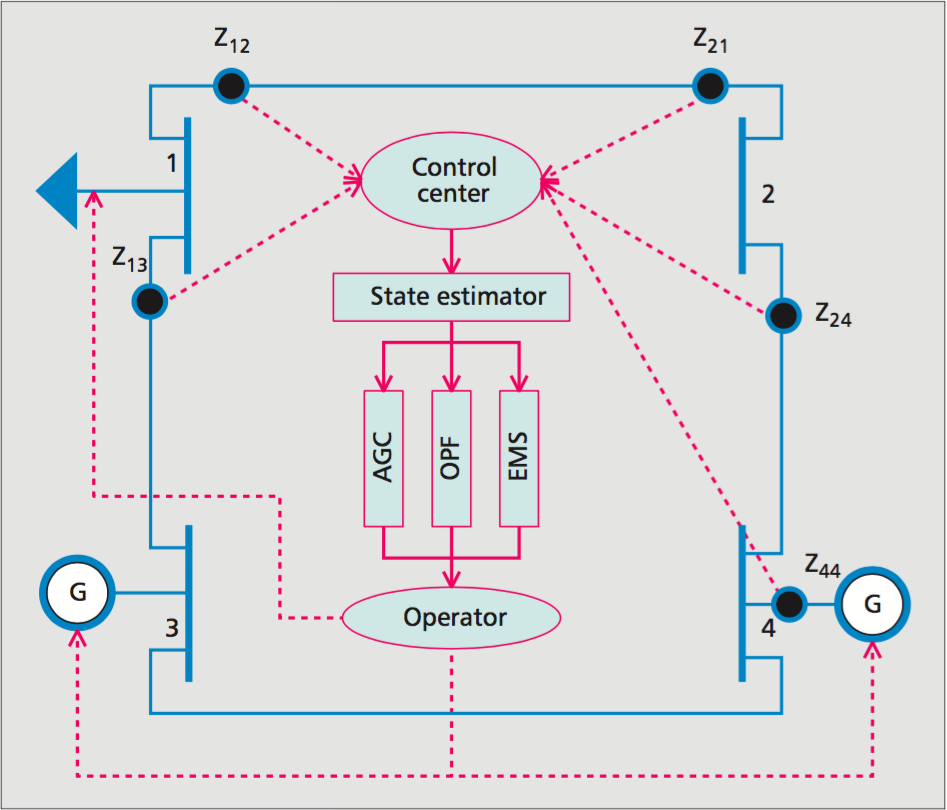
\includegraphics[scale=.3]{imgs/attack/fourbuspowernet.png}
	\caption{Illustrazione di una rete elettrica a quattro bus, centro di controllo, varie funzioni principali (AGC, OPF, EMS), e l'operatore. G rappresenta un generatore, il punto nero rappresenta misurazioni attive sul flusso di corrente ed il triangolo sul bus rappresenta il carico della regione o città.}
	\label{fourbuspowernet_img}
\end{figure}

\subsection{Stima dello stato e Bad Data Injection}
I sistemi elettrici in generale consistono di tre sottosistemi: generazione, trasmissione e distribuzione. Le linee di trasmissione sono utilizzate per trasmettere la corrente elettrica generata ai consumatori. In teoria, la corrente complessiva trasmessa tra il bus \emph{i} ed il bus \emph{j} dipende dalla differenza di voltaggio tra i due bus, ed è funzione dell'impedenza tra questi bus. In genere, le linee di trasmissione hanno un alto rapporto reattanza/resistenza ($X/R$), e quindi l'impedenza di una trasmissione può essere approssimata con la sua reattanza. La corrente attiva trasmessa dal bus \emph{i} al bus \emph{j} può essere scritta come 
\\
\\
\indent$P_{ij} = \frac{V_{i}V_{j}}{X_{ij}}sin(\theta_{i} - \theta_{j})$,
\\
\\
dove $V_{i}$ è la tensione, $\theta_{i}$ è l'angolo di fase del voltaggio nel bus \emph{i}, ed $X_{ij}$ è la reattanza della linea trasmissiva tra il bus \emph{i} ed il bus \emph{j}.\\
Negli studi del flusso di corrente DC (che in questo caso sta per linearità delle equazioni piuttosto che corrente diretta), solitamente si assume che le differenze di fase tra due bus siano piccole, e che le ampiezze dei voltaggi nei bus siano vicine all'unità (dopo essere state normalizzate). Per cui, un'ulteriore semplificazione porta ad una relazione lineare tra gli angoli di fase e la reattanza delle linee,
\\
\\
\indent$P_{ij} = \frac{\theta_{i}\theta_{j}}{X_{ij}}$.
\\
\\
Negli studi sui flussi di potenza, l'angolo di fase del voltaggio ($q_i$) del bus di riferimento è fissato e noto; quindi, solamente $n - 1$ angoli devono essere stimati. I vettori di stato sono definiti come $\textbf{x} = [\theta_1, \ldots, \theta_n]^T$, cioè il vettore degli $n$ angoli di fase dei bus $\theta_i, i = 1, \ldots, n$.\\
Il problema della stima dello stato consiste nello stimare gli $n$ angoli di fase $\theta_i$, osservando $m$ misure in tempo reale, denotate dal vettore $\textbf{z}$ al centro di controllo. Queste misure potrebbero essere sia di corrente attiva trasmessa dal bus $i$ al bus $j$, $P_{ij}$, sia di corrente attiva al bus $i$, $P_i$. La corrente attiva iniettata nel bus $i$ è la super composizione della corrente trasmessa tramite le linee connesse al bus $i$ come $P_i = \sum_j{P_{ij}}$. Il vettore delle osservazioni $\textbf{z}$ può essere descritto come $\textbf{z} = \textbf{h(x)} + \textbf{e}$, dove $\textbf{h(x)}$ è la relazione non lineare tra le misure $\textbf{z}$ e lo stato del sistema $\textbf{x}$, ed $\textbf{e} = [e_1, \ldots, e_m]^T$ è il vettore del rumore Gaussiano delle misure con matrice di covarianza $\Sigma_e$.\\
La matrice del Jacobiano $\textbf{H} \in {\rm I\!R}$ è definita come\\
\indent$\textbf{H}=\frac{\partial\textbf{h(x)}}{\partial\textbf{x}}|_{x=0}$.\\
Se la differenza di fase è piccola, il modello di approssimazione lineare della misura di corrente può essere descritto come\\
\indent Misura sotto Operazioni Normali: $\textbf{z} =  \textbf{Hx} + \textbf{e}$.\\
Da notare che $\textbf{H}$ è generalmente sconosciuta agli attaccanti ma nota all'ISO. Date le misure sul flusso di corrente, il vettore di stato stimato $\widehat{x}$ può essere computato come $\widehat{\textbf{x}} = (\textbf{H}^T\sum_e^{-1}\textbf{H})-1\textbf{H}^T\sum_e^{-1}\textbf{z}$.\\
La Figura \ref{fourbuspowernet_img} mostra il sistema di test a quattro bus della IEEE: ogni bus ha il corrispondente voltaggio ($V_q$) e l'angolo di fase ($\theta_q$); il centro di controllo invia i dati delle misurazioni ($z_{qr}$) ed in seguito lo stimatore di stato inferisce gli stati del sistema che possono essere utilizzati in differenti funzioni, come ad esempio il controllo della generazione automatico (AGC), il flusso di controllo ottimale (OPF), ed il sistema di gestione dell'energia (EMS). L'operatore effettua la decifsione finale per il controllo dei generatori e la gestione del carico (per bilanciare la fornitura e la domanda).
\subsection{Bad Data Detection}
Nella stima dello stato di un sistema elettrico, i ``bad data" come ad esempio bias di misurazione, derive di misura o connessioni errate devono essere identificate. Con il \emph{bad data injection}, gli attaccanti possono iniettare dati all'interno del vettore di misure $r$ ed il sistema può essere descritto come\\
\indent Misura sotto Attacco non-Stealth: $\textbf{z}^\prime = \textbf{H}(\textbf{x}) + \textbf{b} + e$, $\textbf{a} = I\textbf{b}$.\\
Si definisce il vettore residuo $\textbf{r}$ come la differenza tra le qualità misurate ed i valori calcolati dagli stati stimati, precisamente, $\textbf{r} = \textbf{z} - \textbf{H}\widehat{\textbf{x}}$. La media e la covarianza del residuale sono rispettivamente $E(\textbf{r}) = 0$, e $cov(\textbf{r}) = I\sum_{\epsilon}$, dove $I = \textbf{I} - \textbf{M}$, ed $\textbf{M} = \textbf{H}(\textbf{H}^T\sum_e^{-1}\textbf{H})-1\textbf{H}^T\sum_e^{-1}$.\\
I minimi quadrati pesati dell'errore di misura $r^{T}\sum_{e}^{-1}r$ seguono la distribuzione del chi-quadro con $n - m$ gradi di libertà \cite{monticelli}. L'ipotesi a riguardo del rilevamento dei dati fasulli può essere espressa come, $\textbf{r}^T\sum_{e}^{-1}\textbf{r} \ggll \chi_{n-m}^{2},\zeta$, dove $\zeta$ è la probabilità della confidenza del rilevamento.\\
I residuali normalizzati, di tutte le misure, sono utilizzati per identificare i ``bad data". Se la misura corrispondente al maggior residuale normalizzato è maggiore di una soglia di identificazione fissata $\gamma$, \\
\indent $max_i(|\textbf{r}_i|/\sqrt{cov(\textbf{r})}) \geq \gamma$,\\
allora quella misura è considerata come un dato fasullo ed è eliminato dalla stima dello stato.
\subsection{Stealth Bad Data Injection}
Utilizzando lo schema di rilevamento discusso precedentemente, il centro di controllo può difendersi da attacchi \emph{naive} di data injection ed identificare la sorgente di dati corrotti. Questo tipo di attacchi sono chiamati \emph{non stealth}. Però, se un attaccante ha conoscenza della topologia \textbf{H}, può iniettare dati fasulli della forma $\textbf{H}\delta\textbf{x}$ nella misura $\textbf{r}$, più precisamente,\\
\indent Misura sotto Attacco Stealth: $\textbf{z}^\prime = \textbf{H}(\textbf{x} + \delta\textbf{x}) + e$.\\
In questo caso, il test dell'ipotesi fallirebbe il rilevamento dell'attaccante, ed il centro di controllo crederebbe che il vero stato sia $\textbf{x} + \delta\textbf{x}$. Questa è chiamata \emph{stealth bad data injection}. Un'assunzione critica per la fattibilità di questo tipo di attacchi è la disponibilità di informazione completa sulla topologia. Tale assunzione può essere rilassata dal punto di vista dell'attaccante.
\subsection{Meccanismo Difensivo}
La strategia difensiva presentata in \cite{baddatainjattackdef} si basa sull'analisi statistica online della sequenza di dati simultanea al controllo del ritardo di rilevamento e la probabilità di errore entro i livelli desiderati. I metodi di stima dello stato convenzionali \cite{convdef1}, \cite{convdef2} per la \emph{bad data detection} utilizzano le misure per bilanciare il tasso di falsi allarme o il rapporto dei rilevamenti persi. Invece, l'approccio presentato in \cite{baddatainjattackdef} punta a minimizzare il delay di rilevamento soggetto al vincolo sulla probabilità di errore.\\
Si rappresenti con $z_t$ il vettore di osservazioni $m$-dimensionale al tempo $t$. In assenza di un avversario, $z_t$ può essere modellato, per trattabilità, come una distribuzione Gaussiana multivariata a media zero $\mathcal{N}(0, \sum_z)$. Si assume che l'avversario sia inattivo inizialmente; ad un tempo casuale sconosciuto $t$, diventa attivo ed inietta dati malevoli. L'ipotesi binaria può essere formulata come $\mathcal{H}_0: \textbf{Z}_t \sim \mathcal{N}(0, \sum_t)$ ed $\mathcal{H}_1: \textbf{Z}_t \sim \mathcal{N}(\textbf{a}_t, \sum_z)$, dove $\textbf{a}_t = [a_{t,1}, a_{t,2}, \ldots, a_{t,m}]^T \in R^m$ è il vettore dei dati malevoli sconosciuti iniettati dall'attaccante al tempo $t$, ed $\sum_z$ è $\textbf{H}\sum_x\textbf{H}^T + \sum_e$. In altre parole, si vuole rilevare un cambiamento nella distribuzione da $\mathcal(N)(0, \sum_z)$ a $\mathcal(N)(\textbf{a}_t, \sum_z)$ ad un tempo non noto $t$ con $\textbf{a}_t$ sconosciuto.\\
Sia $T_h$ lo \emph{stopping time}, il tempo in cui viene rilevato il cambiamento. Se $T_h < \tau$, è un falso allarme. La lunghezza di esecuzione media (ARL) è $T_d = E[T_h - \tau]$. Basandosi sulla formulazione di Lorden \cite{lorden}, è possibile minimizzare il delay nel caso peggiore, che può essere descritto come $T_d = sup_{\tau \geq 1} E_{\tau}[T_h - \tau | T_d \geq \tau]$. Per computare il minimo $T_d$, l'algoritmo CUSUM di Page è la miglior tecnica per affrontare questo tipo di problemi \cite{lorden}. La maggior parte dei modelli basati su CUSUM assume la conoscenza perfetta delle funzioni di likelihood. Nella detection della bad data injection, i parametri della distribuzione $\mathcal{H}_1$ non possono essere completamente definiti a causa dei parametri degli attaccanti e del modello statistico che non sono noti. Per cui, bisogna progettare meccanismi per il più rapido rilevamento in presenza di parametri non noti.\\
Il CUSUM test adattivo è ricorsivo per sua natura. Ogni ricorsione comprende due step interfogliati:
\begin{itemize}
	\item test CUSUM multi-thread
	\item risolutore lineare di parametri non noti
\end{itemize}
Il CUSUM test multi-thread estende l'algoritmo di Page. Esso considera il tasso di likelihood di $m$ misure a tempo $t$ così da determinare il tempo di stop $T_h$, che può essere descritto come $T_h = Inf\lbrace t \geq 1 | S_t > h \rbrace$, in cui la soglia di rilevamento $h$ è una funzione del tasso di falso allarme (FAR), del tasso di rilevamenti persi (MDR), e la varianza del processo, con statistiche cumulative al tempo $t$: $S_t = max_{1\geq k \geq T_h}\sum_{t=k}^{T_h}$, con $L_t$ pari alla somma della funzione del tasso di likelihood per tutte le misure $(z_{t,j}, j \in \lbrace1, 2, \ldots, m\rbrace)$ al tempo $t$. È possibile esprimere $L_t(\textbf{Z}_t)$ come\\
\indent $\sum_{j=1}^{m}log\frac{f_1(z_{t,j})}{f_0(z_{t,j})}$,\\
dove $f_1(z_{t,j})$ e $f_0(z_{t,j})$ corrispondono alla distribuzione della $j$-esima osservazione al tempo $t$ sotto attacco. Al tempo $t$, la statistica cumulativa $S_t$ può essere risolta ricorsivamente come $max[0, S_{t-1} + L_t(\textbf{Z}_t)]$, dove $S_0 = 0$ quando $t = 0$. Il centro di controllo fa scattare un allarme quando l'accumulazione supera una determinata soglia $h$.\\
\begin{figure}[h]
	\centering
	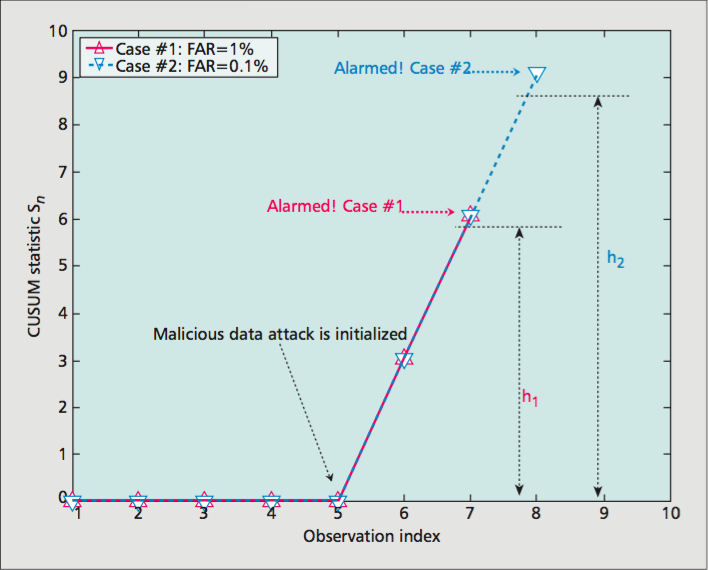
\includegraphics[scale=.3]{imgs/attack/adaptive_CUSUM.png}
	\caption{Il test CUSUM adattivo con intervallo di decisione.}
	\label{cusum_img}
\end{figure}
A causa di un modello statistico avversario sconosciuto, il test del tasso di likelihood generalizzato (GLRT) può essere utilizzato nell'algoritmo CUSUM di Page \cite{lorden}. L'idea è quella di applicare GLRT sostituendo il parametro sconosciuto secondo la stima a maximum likelihood. Quindi, l'espressione ricorsiva del CUSUM test non è più valida in quanto GLRT ha bisogno di computare ogni elemento non noto di ogni misurazione al tempo $t$ stimandolo dalle osservazioni fino al tempo corrente $t$. In altre parole, GLRT richiede la memorizazione delle osservazioni e l'esecuzione della stima ML dei parametri sconosciuti ad ogni punto temporale. Per cui, GLRT è troppo costoso computazionalmente da implementare in pratica per effettuare rilevamento veloce.\\
Per ridurre la complessità computazionale, è possibile applicare il test Rao \cite{lorden}, che è un modello di test asintoticamente equivalente a GLRT. Il Rao test computa le derivate rispetto al parametro non noto valutato in zero, e può essere implementato efficientemente. Inoltre, il Rao test non coinvolge la complessa computazione della stima a maximum likelihood.\\
\subsection{Strategia di attacco}
Gli attacchi stealth sono attuabili quando gli attaccanti hanno piena conoscenza della topologia. Una domanda importante che sorge spontanea è: \textit{se la topologia non è disponibile, può un attaccante effettuare comunque stealth bad data injection?} Sorprendentemente, \textit{si}. L'idea principale presentata in \cite{esmalifalak}, si basa su parametri del sistema variabili in un piccolo range dinamico, infatti, l'informazione sulla topologia è incorporata nelle correlazioni tra le misure di flusso di potenza. Siano $\textbf{z}(t)$ e $\textbf{x}(t)$ le misure ed i vettori di stato al tempo $t$, dove $\textbf{x}(t)$ è sconosciuto. Ad un certo tempo $t$, è impossibile inferire $\textbf{H}$ solamente a partire da $\textbf{z}(t)$. Comunque, con il passare del tempo, e la conoscenza delle proprietà stocastiche del processo casuale $\textbf{x}(t)$, si potrebbe essere in grado di inferire \textbf{H}.\\
Nei sistemi elettrici, le variabili di stato sono generalmente una funzione non lineare dei carichi \textbf{y} e della topologia \textbf{H: x = } \emph{f}(\textbf{y, H}). Mentre la topologia è nota per essere statica in un determinato periodo temporale, i carichi possono essere modellati come \textit{indipendentemente} variabili. Se tali variazioni sono sufficientemente piccole, \emph{f} può essere approssimata utilizzando $\textbf{x} = \textbf{Ay}$, dove \textbf{A} è la matrice dei coefficienti di primo ordine dell'espansione di Taylor in \textbf{y} ($\textbf{z = HAy + e}$).\\
Con \textbf{HA} ed \textbf{y}, è possibile portare a compimento l'attacco modificando i dati misurati come $\textbf{z}^\prime + \textbf{HA}\delta\textbf{y}$, dove $\delta\textbf{y}$ è scelto arbitrariamente. 
Il vettore di stato è stimato come $\widehat{\textbf{x}} = (\textbf{H}^T\sum_e^{-1}\textbf{H})-1\textbf{H}^T\sum_e^{-1}\textbf{z}^\prime$. Sia $\delta\textbf{x} = A\delta\textbf{y}$. Siccome $r = \textbf{z}^\prime - \textbf{H}\wedge x = \textbf{z} + \textbf{H}(\widehat{\textbf{x}} + \delta\textbf{x}), E(\textbf{r}) = 0, cov(\textbf{r}) = (\textbf{I} - \textbf{M})\sum_e$. In altre parole, la media e la varianza di \textbf{r} sono le stesse del caso senza attaccanti. Quindi, utilizzando il metodo del residuale massimo, l'attacco non può essere rilevato.\\
Per inferire \textbf{HA} ed \textbf{y}, è possibile adottare la tecnica della \emph{linear independent component analysis} (ICA). La Linear ICA \cite{lica} è un metodo sviluppato di recente che ha lo scopo di trovare una rappresentazione lineare dei dati cosicché le componenti siano quanto più statisticamente indipendenti possibile. È un caso speciale della \emph{blind source separation}, formulata come segue.
\indent $\textbf{u} = \textbf{Gv}$,\\
con $\textbf{u} = [u_i, i = 1,2, \ldots, m]$ che è il vettore delle osservazioni degli $m$ segnali di monitoraggio, $\textbf{G} = [g_{ij}, i = 1, 2, \ldots,m, j = 1 ,2, \ldots, n]$ è la matrice di mixing non nota, e $v = [v_i, i = 1, 2, \ldots, n]$ è il vettore delle $n$ variabili indipendenti latenti.\\
Dato il modello e la realizzazione di \textbf{u}, ICA può inferire siala matrice di mixing \textbf{G} che il vettore \textbf{v} calcolando in maniera adattiva il vettore dei pesi \textbf{w} che massimizza una misura di \emph{non Gaussianità} del $\textbf{w}^T\textbf{u}$ calcolato.\\
L'algoritmo è mostrato in Figura \ref{algo1}: FastICA \cite{lica}, alla riga 1, è un algoritmo popolare ed efficiente per la ICA che iterativamente trova la direzione in cui il vettore dei pesi \textbf{w} massimizza la non Gaussianità della proiezione $\textbf{w}^T\textbf{z}$ per i dati \textbf{z}. \textbf{G} deve soddisfare $\textbf{w}^T\textbf{G} = \textbf{I}$, con \textbf{I} matrice identità. Le entrate di \textbf{G} minori di una certa soglia $\epsilon$ sono rimosse. Infine, il vettore di stato \textbf{y} può essere stimato da $\textbf{w}^T\textbf{z}$.\\
La riga 2 verifica che \textbf{z} segua un modello lineare. Se le assunzioni di linearità sono valide, $max(\textbf{z} - \textbf{Gy})$ dovrebbe essere piccolo.\\
La riga 3 genera un attacco random tramite una variabile casuale Gaussiana, ed è aggiunto alla variabile inferita \textbf{y} alla riga 4, risultando così in un attacco stealth che non può essere rilevato.
\begin{figure}[htbp]
	\centering
	\fbox{\begin{minipage}{15em}
		Input: \textbf{z} = data matrix
		\begin{enumerate}
			\item $\lbrack \textbf{G}$ and $\textbf{y} \rbrack$ = FastICA(\textbf{z})
			\item If max(\textbf{z} - \textbf{Gy})  $>$ $\epsilon$ then exit
			\item Generate $\delta$\textbf{y} $\sim N(0, \sigma^2)$
			\item $\textbf{z}^\prime$ = \textbf{z} + \textbf{G}(\textbf{y} + $\delta$\textbf{y})

		\end{enumerate}
		Output: false data $\textbf{z}^\prime$
		\end{minipage}
	}
	\caption{Stealth false data injection.}
	\label{algo1}
\end{figure}	

%%%%%%%%%%%%%%%%%%%%%%%%%%%%%%%%%%%%%%%%%%%%%%%%%%%%%%%%%%%%%%%%%%%%%%%%%%%%%%%%%
\section{Disconnect Attack}
Gli smart meter sono la parte più visibile della transizione verso la moderna Smart Grid. Questi sono tipicamente controllati ed interrogati attraverso comunicazioni wireless o su power-line: tali comunicazioni e possibilità di controllo remoto introducono potenziali fonti di attacco con conseguenze gravi per i consumatori ed i proprietari delle infrastrutture.\\
In particolare, lo switch di servizio e la possibilità di connessione/disconnessione remota (RCD) associata degli smart meter, ha colpito l'attenzione della comunità della sicurezza negli ultimi anni \cite{offswitch}, \cite{remotecontrol}, \cite{amithreats}. Un attacco RCD potrebbe causare un blackout diffuso su larga scala o addirittura la minaccia di compiere il suddetto attacco in cambio di soldi \cite{offswitch}. Questo tipo di attacco potrebbe potenzialmente danneggiare la rete elettrica o altri carichi elettrici causando deviazioni nel voltaggio o nella frequenza \cite{remotecontrol}. In tutti i casi, un attacco portato a termine avrebbe serie conseguenze politiche ed economiche.\\
Mentre le misure di sicurezza come la cifratura dei dati ed i sistemi di rilevamento delle intrusioni (IDS) offrono un certo livello di protezione per i sistemi AMI, essi non sono d'aiuto nel caso in cui un attaccante sia capace di compromettere il sistema e far eseguire comandi malevoli a centinaia di migliaia (o milioni) di dispositivi.\\
Le contromisure adottate, presenti in letteratura, fanno uso di ritardi casuali per l'esecuzione dei comandi RCD rendendo così la Smart Grid più resistente:\\
\begin{enumerate}
	\item prevenendo rapidi cambiamenti nel carico che potrebbero destabilizzare il sistema elettrico;
	\item dando il tempo di rilevare e fermare un attacco in corso.
\end{enumerate}
Tali meccanismi di ritardo sono tecnicamente fattibili: alcuni meter supportano un ritardo configurabile prima di rispristinare il servizio dopo un guasto \cite{disconnectfaqs}.
\subsection{Modellare attacchi di Remote Disconnect su AMI}
Si descrivono di seguito i modelli del sistema e degli attaccanti utilizzati per studiare le contromisure di \emph{time delay} per attacchi RCD.
\subsubsection{Modello del sistema}
Si consideri il sistema semplificato di una Smart Grid, in Figura \ref{simplesg_img}, in cui una compagnia utilizza un'unità AMI per controllare un insieme di smart meter a casa dei propri clienti. La comunicazione tra l'unità ed il meter è instradata da più \emph{data concentrator unit} (DCU) intermedi, posizionati in \emph{neighborhood area networks} (NANs). L'unità può effettuare richieste di disconnessione, tramite un DCU, di qualunque meter. Il modello permette di astrarre da protocolli, tecnologie di comunicazione e funzionalità di sicurezza disponibili.\\
\begin{figure}[h]
	\centering
	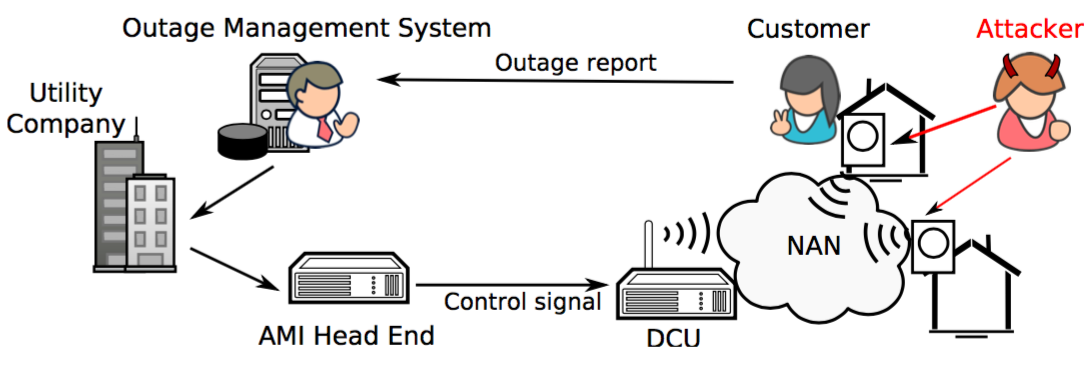
\includegraphics[scale=.3]{imgs/attack/simpleSG.png}
	\caption{Ambiente semplificato. Smart Grid con AMI, sistema di gestione guasti ed un attaccante che sta inviando comandi di disconnessione da remoto ai meter.}
	\label{simplesg_img}
\end{figure}
Il modello del sistema include un \emph{outage management system} (OMS), presso la compagnia, raggiungibile dai clienti tramite telefono o internet. Tale OMS consente alla compagnia di aggregare ed analizzare i report degli utenti.
\subsubsection{Modello dell'attaccante}
Si consideri un attaccante con due scopi possibili:
\begin{enumerate}
	\item denial-of-electrical-service per i clienti di un'azienda durante un determinato periodo di tempo;
	\item disturbo fisico della frequenza della rete elettrica attraverso l'eliminazione del carico.
\end{enumerate}
L'impatto del primo attacco, un attacco di disconnessione su vasta scala in una importante città, può essere devastante ed è discusso in dettaglio in \cite{offswitch}. Oltre questo scenario da caso pessimo, gli attacchi RCD su scala minore (ad esempio a livello del vicinato) possono comunque avere serie ripercussioni, ed essere meno impegnativi per gli attaccanti \cite{amithreats}. Il secondo attacco, la connessione/disconnessione mirata di meter per modificare i parametri del sistema elettrico, discusso in \cite{remotecontrol}. Tale attacco richiederebbe un alto livello di conoscenza del sistema così come un alto numero di dispositivi compromessi.\\
Si modella un attaccante forte per entrambi gli scenari come segue: si assuma che l'attaccante abbia la conoscenza esatta dell'infrastruttura della compagnia (inclusa la topologia di rete, le specifiche degli smart meter e le strategie di controllo) e delle contromisure impiegate dal sistema. L'attaccante può trasmettere messaggi di disconnessione ad ogni meter e tali comandi sono accettati come autentici. Questa astrazione tiene conto di un vasto numero di vettori d'attacco possibili; ad esempio, la compromissione della master key dell'unità AMI, lo sfruttamento di una falla di un protocollo debole e attacchi dall'interno da parte di un operatore AMI. L'attaccante può prevenire la trasmissione di messaggi sul canale di comunicazione primario, se necessario (ad esempio, facendo uso di jammer). L'attaccante è limitato all'interazione con l'unità, DCU e smart meter, inoltre, non può attaccare direttamente l'OMS, la compagnia o canali di comunicazione secondari.
\subsection{Contromisura Delayed Disconnect}
Molte sono le contromisure a disposizione delle compagnie preoccupate per attacchi RCD. Autenticazione e schemi di gestione delle chiavi ben progettati sono componenti essenziali della soluzione, ma in assenza di potenti meccanismi di rilevamento, c'è poco da poter fare nel caso in cui un attaccante ottenga accesso al sistema. I sistemi di \emph{intrusion detection} (IDS) sono un'area di ricerca molto attiva, ma un attaccante potrebbe essere capace di eludere o disabilitare il sistema.\\
Per tale ragione, \cite{delay} concentra la sua attenzione su un altro tipo di contromisura - un delay a tempo casuale per tutte le operazioni RCD. Questo delay dovrebbe essere implementato in ogni smart meter, e la configurazione dei parametri di delay dovrebbe richiedere la presenza fisica per prevenire che un attaccante li modifichi da remoto. Anche se l'IDS o le misure di autenticazione fallissero, questo meccanismo di delay renderebbe la Smart Grid più resistente prevenendo rapidi cambiamenti nel carico e fornendo il tempo necessario al rilevamento di un attacco in corso così da poterlo fermare.\\
Le specifiche dei meccanismi di rilevamento e rispristino dipendono da molti fattori e dal sistema della compagnia. In \cite{delay} è analizzato un meccanismo di rilevamento che comprende il processo di gestione dei guasti della società, come mostrato in Figura \ref{simplesg_img}.\\
Se un attaccante disconnette con successo lo smart meter di un cliente, questo sarà in grado di contattare la compagnia e riferire la perdita di corrente entro un intervallo di tempo ragionevole. Se l'attaccante colpisce un gran numero di clienti, l'OMS della compagnia inizia a ricevere un alto numero di comunicazioni, che innescano un'investigazione. Una volta che l'investigazione stabilisce che i guasti erano di origine malevola, la compagnia può reagire. Si assume che la compagnia sia in grado di far scattare da remoto una modalità \textit{fail-safe}, che cancella tutte le richieste di disconnessione dei meter in sospeso. Questo \emph{trigger} può essere inviato attraverso il canale di comunicazione primario, o nel caso questo sia in controllo dell'attaccante, su un canale secondario. Una possibilità potrebbe essere quella di utilizzare radio secondarie o riconfigurabili \cite{radio}. Un'altra è l'attivazione manuale da parte dell'utente.\\
Ed è proprio la presenza di umani nella rete che rende questa contromisura impegnativa per un attaccante - a patto che il periodo di delay sia lungo abbastanza da far terminare il processo di rilevamento/intervento. Questo fa nascere spontanea la domanda su quanto il delay colpisca le operazioni giornaliere della compagnia, che fa uso di RCD per varie applicazioni.
\subsection{Impatto del delay sui tempi di operazioni RCD}
Si discutono quattro casi d'uso per compagnie RCD (raggruppati in tabella \ref{tab:usecases}) e stimata la loro sensibilità ai time delay. Usando queste stime, sono sviluppate contromisure che migliorano la resistenza del sistema con basso impatto sulle operazioni giornaliere.\\
\subsubsection{Routing Service Switching}
Quando un cliente si trasferisce, la compagnia necessita di fare un \emph{routine service toggling}. Le aziende possono ridurre significativamente i costi operazionali effettuando tali compiti da remoto, piuttosto che inviare tecnici sul luogo. Mentre lo switch del servizio da remoto è portato a termine in minuti \cite{toggle1}, \cite{toggle2}, non è un'operazione particolarmente \emph{time-critical}. Se un'abitazione è stata sgomberata, avrà una richiesta energetica residuale molto bassa. Inoltre, mentre alla comagnia è noto un periodo di trasferimento giorni prima, non lo è l'ora esatta del giorno. Per cui, è ragionevole aspettarsi una finestra RCD di alcune ore.
\subsubsection{Clienti non paganti}
Senza la possibilità di disconnessione da remoto, l'azienda deve disporre di personale addetto alla disconnessione dei clienti non paganti. A volte, questi tecnici sono minacciati quando provano ad accedere al meter. Quindi la disconnessione remota fornisce un guadagno assicurato, così come un beneficio di sicurezza importante. Se un cliente che dispone di uno smart meter \emph{RCD-enabled} non paga le sue bollette, l'azienda può disporre di un ``hard'' switch-off, o di un ``soft'' switch. Così come per il routine service switching, anche questo caso d'uso non è particolarmente time-critical. Senza RCD, potrebbe tranquillamente richiedere ore o addirittura giorni identificare un cliente non pagante, schedulare la disconnessione manuale, e spedire un tecnico in quella particolare area. Per cui questo caso d'uso dovrebbe consentire una finestra RCD di qualche ora.
\begin{table}[hbtp]
	\centering
	\begin{adjustbox}{max width=\textwidth}
		\begin{tabular}{|l|l|l|l|l|}
			\hline
			Num. & Caso d'uso & Beneficio Aziendale & Requisito Temporale & Alternative \\ \hline
			1 & Routine service switching & Risparmi di costi & Ore & Switch Manuale \\ \hline
			2 & Clienti non paganti & Sicurezza del dipendente, garanzia di guadagno & Ore & Switch Manuale\\ \hline
			3 & Limitazione della domanda & Gestione demand-side & Minuti - Ore & Prezzo Dinamico\\ \hline
			4 & Cancellazione dle carico & Controllo del carico a basso livello & Minuti - Ore & Interruttori delle sottostazioni\\ \hline
		\end{tabular}
	\end{adjustbox}
	\caption{Casi d'uso per Smart Meter Remote Connect/Disconnect}
	\label{tab:usecases}
\end{table}
\subsubsection{Limitazione della domanda}
Molti meter supportano una modalità \emph{demand limiting}, che penalizza clienti (sia attraverso la disconnessione o forzando un prezzo più alto dell'elettricità) che eccedono un livello massimo predefinito. È importante tenere presente che la domanda è definita come il carico del cliente in media su un determinato periodo di tempo \cite{demand}. In pratica, questo intervallo temporale sarebbe tra i 5 ed i 30 minuti. Se uno smart meter rileva una violazione del limite della domanda, dovrebbe essere capace di eseguire la conseguenza appropriata nel prossimo intervallo. Comunque, delay più lunghi prima dello \emph{shutoff} potrebbero verificarsi in alcuni casi, come ad esempio un governo che imponga un limite obbligatorio per abitazione. In uno scenario del genere, la disconnessione del meter agisce da deterrente più che da meccanismo di response real-time.
\subsubsection{Cancellazione del carico}
Sebbene le compagnie siano sempre state capaci di eliminare il carico aprendo gli interrutori di circuito, la presenza di smart meter RCD-enabled consente di avere una response più precisa. Il tempo d'esecuzione richiesto per la cancellazione del carico differisce in funzione dell'applicazione. Ad esempio, in situazioni di emergenza la compagnia deve essere in grado di eliminare il carico in real-time. In un sistema con carenze di forniture che necessita di andare in blackout, gli smart meter RCD-enabled consentono un preciso controllo del carico con vincoli temporali meno stringenti.
\subsection{Progettazione delle contromisure di delay}
Introdurre delay prima dell'esecuzione di comandi RCD dovrebbe avere un basso impatto sui casi d'uso visti nella sezione precedente, finché il delay è tenuto al di sotto di una certa soglia. Questo delay massimo è indicato da $d_{max}$, che è variabile dalle decine di minuti alle 2 ore circa, in base agli scenari. Si vede ora come usare questo periodo di delay per migliorare la capacità di recupero della Smart Grid.\\
\subsubsection{Contromisura Delay: il modello}
Si consideri una compagnia con $n$ RCD-enabled smart meter. Lo scopo dell'azienda è di minimizzare il numero totale di meter disconnessi progettando una distribuzione appropriata dei delay temporali su $[0, d_{max}]$. Come anticipato nel Modello del sistema, si considera un processo di rilevamento che coinvolge un sistema di gestione delle interruzioni, che riceve comunicazioni sui guasti da parte degli utenti. \cite{delay} sviluppa due modelli per il processo di rilevamento da parte del OMS, con differenti livelli di astrazione: un modello semplificato per la valutazione analitica, ed un altro più dettagliato da utilizzare all'interno di simulazioni.\\
Nel modello semplificato si assume che l'azienda sia capace di rilevare e fermare un attacco in corso entro $d$ minuti $(d < d_{max})$ una volta che $\tau$ meter siano stati disconnessi in una determinata finestra temporale. In questo modello, $d$ include il tempo necessario affinché i clienti interessati (disconnessi) possano segnalare il guasto, ed il tempo necessario alla compagnia per investigare e concludere che sta avvenendo un attacco, ed inviare comandi che fermino tutte le connessioni in maniera \emph{fail-safe}.\\
Nel modello più dettagliato, si assume che l'attacco sia rilevato una volta che siano state ricevute $\tau^\prime$ segnalazioni di guasto da parte dei clienti tramite l'OMS durante un periodo temporale (i tempi di segnalazione individuali sono campionati da una specifica distribuzione).
Quando questa condizione è verificata, l'azienda ha tempo aggiuntivo, $d^\prime$, per investigare prima di inviare comandi \emph{fail-safe}. In ogni caso, il valore di $\tau$ $(o$ $\tau^\prime)$ dovrebbe corrispondere ad una piccola frazione del numero totale di meter, ma deve essere grande abbastanza da escludere la maggior parte dei guasti non relativi alla sicurezza. Il tempo di risposta $d$ $(o$ $d^\prime)$ dovrebbe essere circa dello stesso ordine di $d_{max}$. L'intervallo temporale impostato per il rilevamento in accordo alla finestra temporale dell'obiettivo dell'attaccante, che si assume essere nell'ordine delle ore.
\subsubsection{Meccanismi di delay}
Le performance della contromisura RCD time delay dipende dalla distribuzione del delay, che deve essere progettata contro un attaccante che può selezionare il numero di meter da colpire e pianificare quando inviare i comandi di disconnessione. Si considerino ora, tre distribuzioni di delay: uniforme, Bernoulli e geometrica. Si sviluppano i limiti analitici per il numero di meter che un attaccante può disconnettere con successo seguendo una sua strategia ottimale. La Figura \ref{distributions_img} mostra le funzioni di probabilità densità/massa dei tre meccanismi.
\begin{figure}[hbtp]
	\centering
	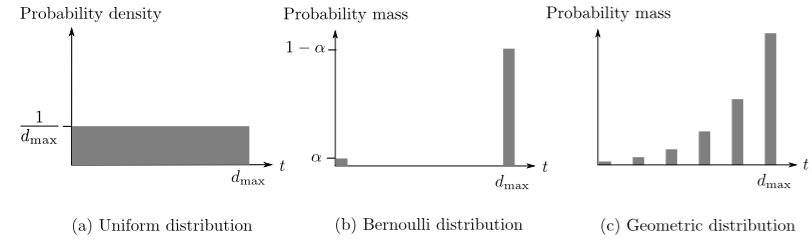
\includegraphics[scale=.45]{imgs/attack/distributions.png}
	\caption{Meccanismi di delay RCD.}
	\label{distributions_img}
\end{figure}
\paragraph{Delay Uniforme.} Secondo questo meccanismo di delay molto basico, una volta che un meter riceve un comando di disconnessione autenticato, esso seleziona un back-off di delay casuale uniformemente da $[0, d_{max}]$. Ogni meter seleziona il suo delay di back-off indipendentemente e si disconnette dopo tale tempo.\\
Si esamini il momento in cui $\tau$ meter si sono appena disconnessi. Secondo il modello di rilevamento e notifica, l'azienda sarebbe in grado di fermare l'attacco entro altri $d$ minuti, annullando tutti i comandi di disconnessione che sono ancora in corso. Durante questi $d$ minuti, l'attaccante può continuare a disconnettere $nd/d_{max}$ meter aggiuntivi in media, assumendo che un attaccante abbia già inviato i comandi di disconnessione a tutti i meter. Siccome non c'è miglior strategia di attacco, questo fornisce un limite superiore al numero totale di meter disconnessi pari a $\tau + dn/d_{max}$, che cresce linearmente con $n$ dato $d/d_{max}$ costante.
\paragraph{Delay Bernoulli.} Una distribuzione alternativa per ridurre il numero di meter disconnessi è la distribuzione di Bernoulli. In pratica, ogni meter lancia una moneta truccata per scegliere tra due possibili intervalli, ognuno di almeno 10 secondi per evitare problemi di stabilità. In particolare, con probabilità $\alpha$ (parametro di sistema), il meter si disconnette quasi immediatamente, Altrimenti, esso pospone la sua disconnessione verso la fine del periodo consentito $(delay \approx d_{max})$. L'intuizione alla base è semplice: se sono attaccati un gran numero di meter, quelli che si disconnettono quasi immediatamente innescherebbero il rilevamento da parte dell'OMS, che a sua volta ferma l'attacco in corso per la maggior parte dei meter che pospongono la disconnessione.\\
In questo caso la miglior strategia per un attaccante è di non inviare comandi di disconnessione a tutti gli $n$ meter in un solo colpo: continuando ad utilizzare questa strategia consentirebbe alla compagnia di impostare $\alpha$ ad un valore molto basso così da ridurre il numero di meter disconnessi. Invece, un attaccante può massimizzare il numero di meter disconnessi lanciando un attacco \emph{two-batch}: l'attaccante sceglie il numero totale di meter in un primo gruppo così che il sottoinsieme di meter disconnessi immediatamente non faccia scattare la notifica. Nel momento in cui il sottoinsieme di meter del primo gruppo che sceglie di posporre inizia a disconnettersi (e notificherà presto all'azienda), l'attaccante invia i comandi a tutti gli altri meter. Sotto un attacco del genere, tutti i meter nel primo gruppo e, ci si aspetta, un sottoinsieme di una frazione $\alpha$ dei meter nel secondo gruppo si sarebbero disconnessi prima che i comandi di disconnessione in attesa siano annullati. Sommando questi due termini otteniamo un limite superiore al numero totale di meter disconnessi pari a $\tau/\alpha + (n - \tau/\alpha)\alpha$. L'azienda potrebbe scegliere strategicamente $\alpha = \sqrt{\tau/n}$ per minimizzare il limite a $2\sqrt{\tau n} - \tau$, che cresce in maniera sublineare in $n$.
\paragraph{Delay Geometrico.} Se il delay RCD massimo $d_{max}$ è poche volte maggiore di $d$, la compagnia può ridurre ulteriormente il numero di meter disconnessi applicando una distribuzione geometrica sui periodi di delay consentiti. Sia $k = [d_{max}/d]$. Con questo meccanismo di delay, un meter sceglierà tra $k$ possibili intervalli, con l'$i$-esimo $(i = 1, \ldots, k)$ intervallo di delay di durata circa $(i - 1)d/d_{max}$ e scelto con probabilità $(\beta^i - \beta^{i-1})/(\beta^k - 1)$. In questo caso, $\beta$ è un parametro di sistema che può essere ottimizzato in accordo a $k$ ed altri parametri (ad esempio $n$ e $\tau$). Si noti che quando $k = 2$, l'ottimizzazione di $\beta$ degenererebbe il meccanismo di delay geometrico nel meccanismo di delay Bernoulliano.\\
Utilizzando questa distribuzione geometrica ed il modello definito in precedenza, a prescindere dalla strategia adottata dall'attaccante, in media meno di $\tau(1+\beta) + (n - \tau)(\beta - 1)/(\beta^k - 1)$ meter sarebbero disconnessi. Il primo termine limita il numero di meter a cui è stato inviato il comando di disconnessione prima che $\tau$ meter siano disconnessi, ed il secondo termine limita il numero di meter a cui è stato inviato il comando di disconnessione dopo di ciò. Con la costante $\beta$, il primo termine cresce linearmente con $\tau$, che è una piccola frazione di $n$, ed il secondo termine decade geometricamente con $k$, che sarà anch'esso una piccola frazione di $n$, anche per piccoli valori di $k$.
\paragraph{Riepilogo.}
\begin{figure}[hbtp]
	\centering
	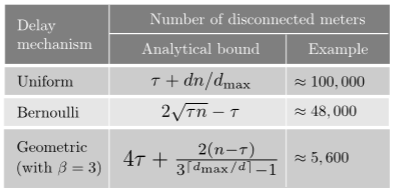
\includegraphics[scale=.5]{imgs/attack/dist_perf.png}
	\caption{Riepilogo dell'analisi con un setting d'esempio di $d = 10$ min, $d_{max} = 60$ min, $\tau = 1000$ ed $n = 600.000$.}
	\label{dist_perf_img}
\end{figure}
La Figura \ref{dist_perf_img} riassume i risultati analitici per i tre meccanismi di delay. Per ognuno di essi, il numero di meter disconnessi cresce ad un tasso asintotico differente rispetto ad $n$. Come illustrato nel setting d'esempio, secondo il meccanismo di delay geometrico, fin quando $d_{max}$ è poche volte (ad esempio, $6\times$) maggiore di $d$, il numero di meter disconnessi sarà piccolo $(< 1\%$ di $n)$. In confronto, secondo il meccanismo di delay uniforme, un numero significativamente maggiore di meter $(> 10\%$ di $n)$ sarebbe disconnesso. Per il meccanismo di delay di Bernoulli, il numero di meter disconnessi è nell'ordine di $\sqrt{\tau n}$, quindi dipende altamente dalla soglia di rilevamento $\tau$. Quando $\tau$ è circa lo $0.2\%$ di $n$ (come nei setting d'esempio), il numero di meter disconnessi può comunque raggiungere circa l'$8\%$ di $n$. Un confronto di questi tre meccanismi di delay suggerisce:
\begin{enumerate}
	\item se possibile, un'azienda dovrebbe rendere $d_{max}$ svariate volte maggiore di $d$, ed utilizzare il meccanismo di delay geometrico;
	\item altrimenti, se $\lceil d_{max}/d \rceil = 2$ ed il meccanismo di distribuzione geometrico degenera al Bernoulliano, la compagnia deve portare la sua soglia di rilevamento $\tau$ al valore minore possibile per favorire la propria capacità di recupero sotto attacchi RCD.
\end{enumerate}
%%%%%%%%%%%%%%%%%%%%%%%%%%%%%%%%%%%%%%%%%%%%%%%%%%%%%%%%%%%%%%%%%%%%%%%%%%%%%%%%%
\section{Replay Attack}
%%%%%%%%%%%%%%%%%%%%%%%%%%%%%%%%%%%%%%%%%%%%%%%%%%%%%%%%%%%%%%%%%%%%%%%%%%%%%%%%%
\section{Jamming}
L'infrastruttura di comunicazione svolge un ruolo predominante nelle Smart Grid. Si occupa principalmente di broadcast real-time del prezzo della corrente, di riportare i consumi energetici e di monitorare lo stato del sistema. Grazie allo scambio di informazioni in tempo reale un utente è in grado di determinare il proprio consumo energetico ottimale.\newline
Così come i vantaggi, l'infrastruttura di comunicazione presenta alcune vulnerabilità. In questa sezione, si analizza in dettaglio una strategia di attacco che manipola il mercato elettrico utilizzando la tecnica del \emph{Jamming}. Questo attacco causa cambiamenti nei consumi energetici e tende quindi a destabilizzare le power grid (vedi Figura \ref{fig:jm}). 
\begin{figure}[h]
	\centering
	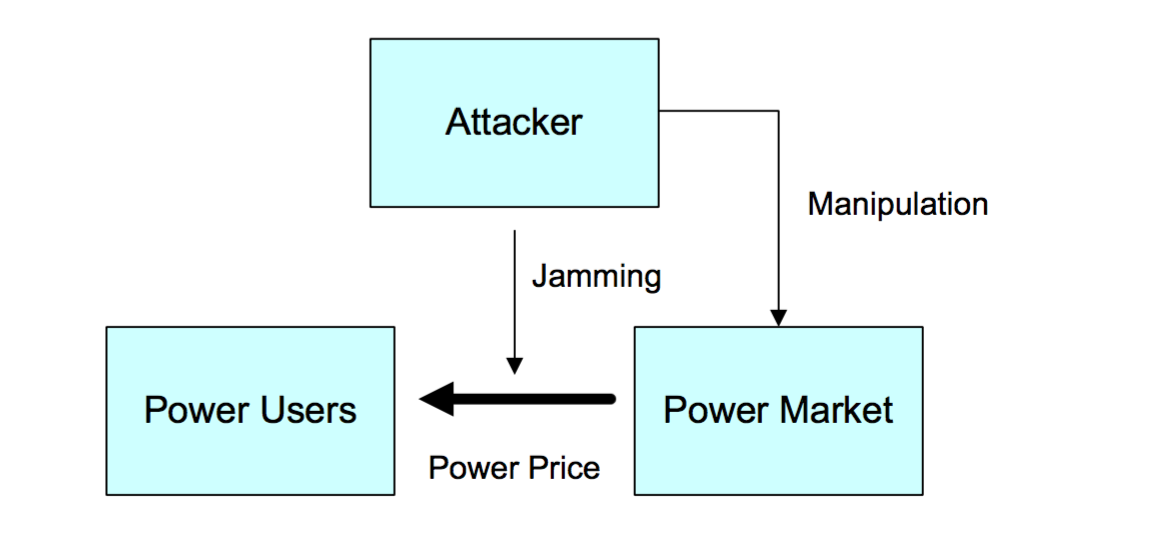
\includegraphics[scale=0.320]{imgs/attack/jm.png}
	\caption{Un'illustrazione della manipolazione del mercato attraverso il Jamming} \label{fig:jm}
\end{figure}\\
Si assume che è utilizzato un sistema di comunicazione wireless, come WiMAX, per effettuare il broadcast delle informazioni relative ai prezzi. Un attaccante, utilizzando un jammer molto potente in un'area abbastanza vasta, disturba l'invio real-time dei prezzi. Si assume che ogni consumer continua a far riferimento al vecchio prezzo in quanto le informazioni aggiornate sul prezzo non arrivano a destinazione. L'attaccante continua a fare jamming fin quando non c'è una variazione reale sul prezzo. Una volta ricevuto il nuovo prezzo, gli utenti coinvolti modificheranno e/o si adegueranno, causandone una diminuzione o un incremento, facile da predire. In questo modo un attaccante può cambiare il prezzo della corrente quando e nella direzione in cui vuole.
\subsection{Modello del sistema}
Si considera una power grid con $N$ bus. Ogni bus è connesso ad un generatore elettrico. Sul bus \emph{n}, la corrente generata è denotata da \emph{$G_{n}$} e il costo unitario per la generazione è indicato con \emph{$C_{n}$}. Si assume vi siano \emph{M} utenti su ogni bus. L'$m$-esimo utente sul bus $n$ ha un consumo energetico $d_{nm}(t)$ nello slot temporale \emph{t}. Il consumo energetico totale sul bus \emph{n} è dato da $D_{n} = \sum_{m=1}^{M}d_{nm}$. Ci sono \emph{K} linee di trasmissione. L'upper bound realativo alla corrente trasmessa sulla linea \emph{k} è denotato con $F_{k}^{max}$. Il generation shift factor dal bus \emph{n} alla linea di trasmissione \emph{k} si indica con $GSF_{n \rightarrow k}$ se quel bus è adiacente a tale linea. Un esempio della power grid con 5 bus è mostrato in Figura \ref{fig:pjm}.
\begin{figure}[h]
	\centering
	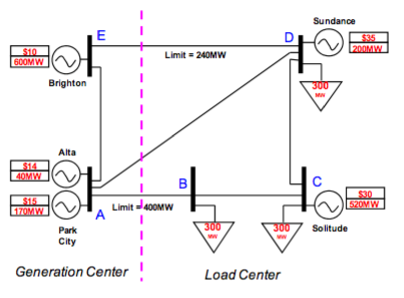
\includegraphics[scale=0.400]{imgs/attack/pjm.png}
	\caption{Un'illustrazione di un sistema PJM con 5 bus} \label{fig:pjm}
\end{figure}
\newpage
La generazione di corrente è determinata dal seguente problema di programmazione lineare\cite{jam}.
\begin{equation*}
\begin{array}{ll@{}ll}
\text{min}  & \displaystyle\sum\limits_{n=1}^{N} C_{n} \times G_{n} &\\
\text{s.t.}& \displaystyle\sum\limits_{n=1}^{N} G_{n} -  \sum\limits_{n=1}^{N} D_{i} = 0,&\\
               & GSF_{n \rightarrow k} \times (G_{n} - D_{n}) \leq F_{k}^{max},\forall k&\\
\end{array}
\end{equation*}
Si assume che il consumo energetico è determinato da un'utility function relativa al consumer, denotata con $U(w,d)$, in cui $w$ rappresenta l'internal power requirement e $d$ rappresenta il consumo. Si assume che questa funzione cresce con l'aumentare di $d$ e decresce con l'aumentare di $w$. Inoltre, si assume che il guadagno di un utente è dato da $R(w,d,p) = U(w,d) - dp$, che è il valore della funzione a cui si va a sottrarre il prezzo relativo al consumo energetico. Quindi, il livello di consumo energetico ottimale dovrebbe massimizzare il guadagno totale $d^{*} = arg max \Big[U(w,d) - dp\Big]$ al variare di $d$. Per semplicità si può pensare che tutti gli utenti hanno la stessa utility function. Si assume anche che il consumo energetico ottimale è funzione continua, decrescente e convessa del prezzo, dato un fissato valore $w$. La randomness sui consumi deriva dalla randomness relativa all'internal power requirement caratterizzata dal parametro $w$. Si assume che $w$ sia una catena di Markov, che ha $L$ valori $w_{1} \leq w_{2} \leq w_{3} \leq \cdots \leq w_{L}$. La probabilità di transizione di stato è denotata con $p_{nm}$ per gli stati $n$ e $m$ e può avvenire solo tra stati adiacenti.
\newpage
\subsection{Strategia di attacco}
Descrizione relativa alla procedura d'attacco:
\begin{enumerate}
	\item L'attaccante fa jamming in un'area molto popolata;
	\item L'utente coinvolto è a conoscenza del vecchio prezzo della corrente dal momento in cui il nuovo prezzo non gli è noto;
	\item L'attaccante monitora il mercato elettrico e continua a fare jamming;
	\item Nel momento in cui il prezzo cambia significativamente, si smette di fare jamming;
	\item Ogni utente adatta il suo consumo energetico in base al nuovo prezzo. Se il nuovo prezzo è superiore al vecchio, l'utente diminuisce i suoi consumi, facendo calare il prezzo della corrente con alta probabilità. Viceversa, se il nuovo prezzo è più piccolo, un utente incrementa i suoi consumi, aumentando con alta probabilità il prezzo dell'energia;
	\item L'attaccante può avere dei profitti dalla manipolazione del mercato.
\end{enumerate}
\subsection{Impatto}
Si suppone che il bus \emph{n} ha subito jamming. Si denotano con $p_{0}$ e $p_{n}$ il vecchio e il nuovo prezzo, prima e dopo aver cessato il jamming. $\pi_{i}$ è la proporzione di utenti sul jammed bus che sono nello stato $i$. Quando il numero di utenti $M$ nel bus è sufficientemente grande, la proporzione può essere approssimata da una probabilità stazionaria della catena di Markov. Il cambiamento del cosumo energetico totale dopo aver ottenuto il prezzo della corrente è:\newline
\indent$\delta D = \sum\limits_{i=n}^{N} \Big[ d_{l_{n}(t+1)}(p_{n}) - d_{l_{n}(t)}(p_{0})\Big]$,\newline
dove $l_{n}(t)$ è il power requirement index dell'utente $n$ al tempo $t$, $d_{i}$ è la funzione del consumo energetico ottimale quando il power requirement index corrente è $i$. L'expectation sul cambiamento del consumo energetico risulta:\newline
\indent$E[\delta D] = M \sum\limits_{i=1}^{L} \pi_{i} \Big[\sum\limits_{j} P_{ij}d_{j}(p_{n}) - d_{i}(p_{0})\Big]$.\newline\newline
Quando $M$ è sufficientemente grande, il cambiamento del consumo energetico può essere approssimato da una distribuzione Gaussiana, con expectation descritta precedentemente e varianza pari a:\newline
\indent$Var[\delta D] = \sqrt{M} \sum\limits_{i=1}^{L} \pi_{i} \Big\{\sum\limits_{j}P_{ij}d_{j}^{2}(p_{n}) - \Big[\sum\limits_{j}P_{ij}d_{j}^{2}(p_{n})\Big]^2\Big\}$.\newpage
In questo caso si è assunto che $\Delta D > 0$. L'analisi si può anche applicare nel caso $\Delta D < 0$. Se l'attaccante ha un profitto nel momento in cui $\Delta D > \Delta D_{min}$ allora in accordo all'approssimazione Gaussiana, la probabilità che egli riesca nell'attacco è data da $P_{s} \approx 1 - Q \bigg(\frac{\Delta D_{min} - E[\Delta D]}{\sqrt{Var[\Delta D]}}\bigg)$.
\subsection{Contromisure}
A causa dei potenziali gravi danni che questo attacco può infliggere al mercato elettrico, il meccanismo price-response deve essere in grado di impedire un tale attacco. L'essenza della contromisura sta nell'evitare di modificare il consumo di energia in maniera simultanea. L'idea è basata sui protocolli come l'Aloha e CSMA, in cui i diversi trasmettitori utilizzano backoff casuali per evitare le collisioni dovute a trasmissioni simultanee.\newline\newline
E' stato proposto uno schema di backoff casuale, in cui ogni consumer sceglie un tempo casuale per cambiare la propria power response. T è una variabile casuale che dipende dalla differenza tra il nuovo e il vecchio prezzo, denotata da $\delta p$, e dal tempo in cui il segnale relativo al prezzo non è stato ricevuto, noto come $\tau$. Si assume che il tempo è esponenzialmente distribuito con\newline
\indent$p(T = t) = (e^{\lambda} - 1) e^{- \lambda t}, t = 1,2,3,\cdots$
\newline
dove $\lambda$ è funzione di $\delta p$ e $\tau$. Se un attaccante ferma il jamming al tempo 0, allora il cambiamento del carico elettrico sul jammed bus nello slot temporale t, confrontato con il carico al tempo 0, è dato da:\newline
\indent$\delta D(t) = \sum\limits_{i=n}^{N} I(T_{n} < t) \Big[d_{l_{n}(t)}(p_{n}) - d_{l_{n}(0)}(p_{0})\Big]$,
\newline
con expectation:\newline
\indent$E[\delta D] = P(T \leq t) \times M \sum\limits_{i=1}^{L} \pi_{i} \Big[\sum\limits_{j} P_{ij}^{t}d_{j}(p_{n}) - d_{i}(p_{0})\Big]$,\newline
dove $P_{ij}^{t}$ è la probabilità di transizione tra i livelli di consumo $i$ e $j$ dopo $t$ slot temporali, e varianza:\newline
\indent$Var[\delta D] = P(T < t) \times \sqrt{M} \sum\limits_{i=1}^{L} \pi_{i} \Big\{\sum\limits_{j}P_{ij}^{t}d_{j}^{2}(p_{n}) - \Big[\sum\limits_{j}P_{ij}^{t}d_{j}^{2}(p_{n})\Big]^2\Big\}$.\newline
L'idea è quindi quella di diffondere le informazioni relative ai cambiamenti dei consumi energetici in un intervallo di tempo molto più grande lasciando che la randomness intrinseca del mercato possa contrattaccare i cambiamenti dei jammed user.
% \section{Web Application} già discussa nell'OSSTMM
\section{Rilevamento}
\section{Power Fingerprinting}
%\section{Optimal Malicious Attack Construction and Robust Detection in Smart Grid Cyber Security Analysis}


\begin{thebibliography}{99}
\bibitem{standard14908} International Organization for Standardization. ISO/IEC 14908-1:2012:Information technology – Control network protocol – Part 1: Protocol stack, 2012.
\bibitem{wep1} Andreas Klein. \emph{Attacks on the RC4 stream cipher.} Des. Codes Cryptography, 48(3):269–286, 2008.
\bibitem{wep2} Erik Tews, Ralf-Philipp Weinmann, and Andrei Pyshkin. \emph{Breaking 104 bit WEP in less than 60 seconds.} In Sehun Kim, Moti Yung, and Hyung-Woo Lee, editors, Information Security Applications, 8th International Workshop, WISA 2007, Jeju Island, Korea, August 27-29, 2007, Revised Selected Papers, volume 4867 of Lecture Notes in Computer Science, pages 188–202. Springer, 2007.
\bibitem{aircrackng} Aircrack-ng. \url{http://www.aircrack-ng.org/}
\bibitem{kali} Kali Linux. \url{https://www.kali.org/}
\bibitem{wireshark} Wireshark. \url{https://www.wireshark.org/}
\bibitem{nmap} Nmap. \url{https://www.nmap.org/}
\bibitem{nessus} Nessus. \url{https://www.nessus.org/}
\bibitem{cainabel} Cain \& Abel. \url{http://www.oxid.it/}
\bibitem{metasploit} Metasploit. \url{http://www.metasploit.com/}
\bibitem{monticelli} A. Monticelli, ``Electric Power System State Estimation," Proc. IEEE, vol. 88, Feb. 2000, pp. 262–82.
\bibitem{baddatainj} M. Esmalifalak, Z. Han, and L. Song, ``Effect of Stealthy Bad Data Injection On Network Congestion In Market Based Power System," IEEE WCNC 2012, Paris, France, Apr. 2010.
\bibitem{falsedatainj} Y. Liu, M. K. Reiter, and P. Ning, ``False Data Injection Attacks Against State Estimation in Electric Power Grids," 16th ACM Conf. Computer and Commun. Security, Gaithersburg, MD, Nov. 2009, pp. 21–30.
\bibitem{baddatainj2} L. Xie, Y. Mo, and B. Sinopoli, ``False Data Injection Attacks in Electricity Markets," 1st IEEE Int’l. Conf. Smart Grid Commun., Gaithersburg, MD, Oct. 2010, pp. 226–31.
\bibitem{baddatainjattackdef} Huang, Yi, et al. ``Bad data injection in smart grid: attack and defense mechanisms." Communications Magazine, IEEE 51.1 (2013): 27-33.
\bibitem{convdef1} A. Abur and A. G. Exposito, Power System State Estimation: Theory and Implementation, Marcel Dekker, 2004.
\bibitem{convdef2} A. J. Wood and B. F. Wollenberg, Power Generation, Operation, and Control, Wiley, 1996.
\bibitem{lorden} H. V. Poor and Q. Hadjiliadis, Quickest Detection, Cambridge Univ. Press, 2008.
\bibitem{esmalifalak} M. Esmalifalak et al., ``Stealth False Data Injection using Independent Component Analysis in Smart Grid," 2nd IEEE Conf. Smart Grid Commun., Brussels, Belgium, Oct. 2011.
\bibitem{lica} J. Himberg and A. Hyvarinen, ``Independent Component Analysis for Binary Data: An Experimental Study," 3rd Int’l. Conf. Independent Component Analysis and Blind Signal Separation, Malm, Sweden, June 2001.
\bibitem{offswitch} R. Anderson and S. Fuloria, ``Who controls the off switch?" in Proc. of the Conference on Smart Grid Communications (SmartGridComm), 2010.
\bibitem{remotecontrol} M. Costache, V. Tudor, M. Almgren, M. Papatriantafilou, and C. Saunders, ``Remote control of smart meters: friend or foe?" in Proc. of the European Conference on Computer Network Defense (EC2ND), 2011.
\bibitem{amithreats} D. Grochocki, J. H. Huh, R. Bobba, W. H. Sanders, A. A. Cardenas, and J. G. Jetcheva, ``AMI threats, intrusion detection requirements and deployment recommendations," in Proc. of the Conference on Smart Grid Communications (SmartGridComm), 2012.
\bibitem{disconnectfaqs} ``GE I-210+ remote disconnect FAQs," \url{http://www.dbmss.ca/PDF\%20files/I210+_and_I210+c_Remote_Disconnect_FAQ_2.pdf}.
\bibitem{delay} Temple, William G., Binbin Chen, and Nils Ole Tippenhauer. ``Delay makes a difference: Smart grid resilience under remote meter disconnect attack." Smart Grid Communications (SmartGridComm), 2013 IEEE International Conference on. IEEE, 2013.
\bibitem{radio} A. Ghassemi, S. Bavarian, and L. Lampe, ``Cognitive radio for smart grid communications,'' in Proc. of the Conference on Smart Grid Communications (SmartGridComm), 2010.
\bibitem{toggle1} ``Avista utilities update to idaho public utility commission staff on remote reconnect/disconnect pilot,'' \url{http://www.puc.idaho.gov/fileroom/ cases/elec/AVU/AVUE0709/company/20130211UPDATE\%20ON\% 20REMOTE\%20RECONNECT\%20DISCONNECT.PDF}.
\bibitem{toggle2} ``Texas-new mexico power company’s request for approval of an advanced metering system (ams) deployment and ams surcharge,'' \url{http: //www.smartgrid.gov/sites/default/files/doc/files/TexasNew_Mexico_Power_Company_Request_For_Approval_Advance_201005.pdf}.
\bibitem{demand} W. H. Kersting, ``Distribution system modeling and analysis.'' CRC Press, LLC, 2012.
%
%
% avoid conflicts
\bibitem{jam} F. Li and R. Bo, ``Congestion and price prediction under load variation'', IEEE Control System Magazine, vol.19, pp.59–70, Oct. 2009.
\end{thebibliography}